\chapter{Annex 1: Budget}

The budget shown in Figure~\ref{fig:Budget} is divided into three sections:


\begin{enumerate}
	\item The first section reflects the cost of time and resources dedicated to the development of the software from February 3rd (the week I began development) to June 8th (the week I stopped development). Additional weeks and hours spent on writing the report are not included.
	
	\item The second section estimates the cost required to complete the development, resulting in a feature-complete, user-friendly, competitive, and marketable program. This is projected as six months of full-time work (not accounting for holidays or vacations). My hourly rate is also increased, since after the approval of this project, I will no longer be considered a student in training, but rather a junior-level graduate professional, able to dedicate myself fully to the task.
	
	\item The third section lists the audio equipment required to deploy the software on-site and operate it effectively. This equipment falls within the professional range, yet remains reasonably priced for its category. All prices were obtained from a trusted reference retailer in the European market—Thomann\cite{thomann}.
\end{enumerate}

It is generally considered that a laptop should be amortized over a period of two years. Assuming that my laptop and its additional peripherals cost approximately 1500€, and should be amortized across 104 weeks, the resulting cost of using the laptop is approximately 14.43€ per week.

Additionally, a General Expenses category has been included, which mainly covers a proportional share of electricity costs and minor office supplies such as pens, paper, pencils, erasers, screen cleaning fluid, and other similar items.


\begin{figure}[H]
	\centering
	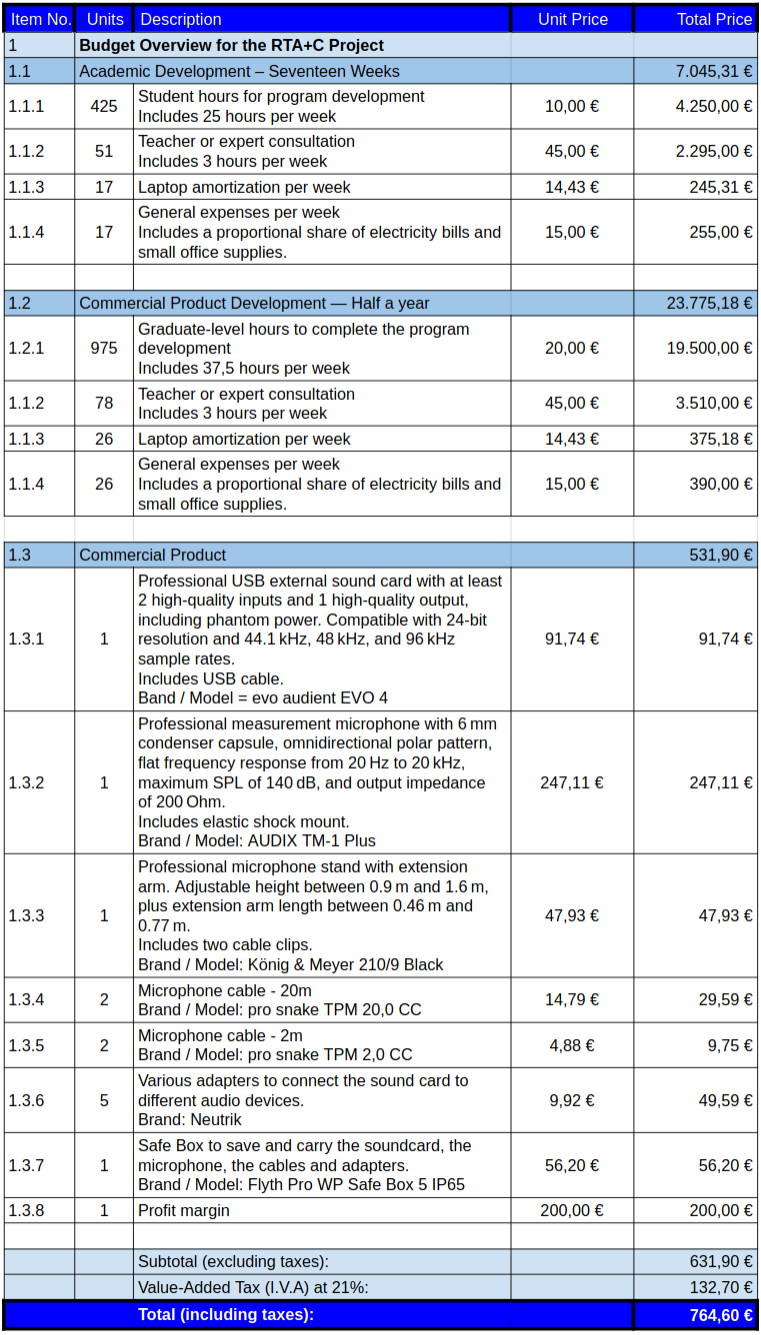
\includegraphics[width=0.82
	\linewidth]{Figures/Budget.png}
	\caption{Budget for the entire project}
	\label{fig:Budget}
\end{figure}

